% Straight up stealing preamble from Eli Holmes 
%%%%%%%%%%%%%%%%%%%%%%%%%%%%%%%%%%%%%%START PREAMBLE THAT IS THE SAME FOR ALL EXAMPLES
\documentclass{article}

%Required: You must have these
\usepackage{Sweave}
\usepackage{graphicx}
\usepackage{tabularx}
\usepackage{hyperref}
\usepackage{natbib}
\usepackage{gensymb}
%\usepackage[backend=bibtex]{biblatex}
%Strongly recommended
 %put your figures in one place
 
%you'll want these for pretty captioning
\usepackage[small]{caption}

\setkeys{Gin}{width=0.8\textwidth} %make the figs 50 perc textwidth
\setlength{\captionmargin}{30pt}
\setlength{\abovecaptionskip}{0pt}
\setlength{\belowcaptionskip}{10pt}
% manual for caption http://www.dd.chalmers.se/latex/Docs/PDF/caption.pdf

%Optional: I like to muck with my margins and spacing in ways that LaTeX frowns on
%Here's how to do that
 \topmargin -2cm     
 \oddsidemargin -0.04cm   
 \evensidemargin -0.04cm  % same as oddsidemargin but for left-hand pages
 \textwidth 16.59cm
 \textheight 22.94cm 
 %\pagestyle{empty}       % Uncomment if don't want page numbers
 \parskip 7.2pt           % sets spacing between paragraphs
 %\renewcommand{\baselinestretch}{1.5} 	% Uncomment for 1.5 spacing between lines
\parindent 0pt% sets leading space for paragraphs
\usepackage{setspace}
%\doublespacing

%Optional: I like fancy headers
\usepackage{fancyhdr}
\pagestyle{fancy}
\fancyhead[LO]{Do early phenological events constrain later phenology?}
\fancyhead[RO]{2017}
 
%%%%%%%%%%%%%%%%%%%%%%%%%%%%%%%%%%%%%%END PREAMBLE THAT IS THE SAME FOR ALL EXAMPLES

%Start of the document
\begin{document}

% \SweaveOpts{concordance=TRUE}
 \bibliographystyle{/Users/aileneettinger/citations/Bibtex/styles/nature.bst}
\title{Do early phenological events constrain later phenology?} 
\author{A.K. Ettinger, S. Gee, and E.M. Wolkovich}
%\date{\today}
\maketitle  %put the fancy title on
%\tableofcontents      %add a table of contents
%\clearpage
%%%%%%%%%%%%%%%%%%%%%%%%%%%%%%%%%%%%%%%%%%%%%%%%%%%

\section* {Goal}
\par We aim to test the extent to which previous phenological stages constrain later ones, as this is poorly understood. We plan to submit this paper as a ``brief communication" at	American Journal of Botany or a ``rapid report" at
New Phytologist.

\section* {Hypotheses}
 %\citep{wolkovich2014}
\par Hypothesis 1: Previous phenological events constrain later events; e.g., late-fruiting species et fruit late in the season because they leaf-out late  (Figure \ref{fig:hyp}).
\par Hypothesis 2: Inter-phenophase time  constrains phenology; e.g., late-fruiting species set fruit late in the season because they require longer development time (Figure \ref{fig:hyp}).

\section* {Main Messages}
Main messages for Sally's thesis paper
\begin{enumerate}
\item Earlier phenological stages constrain later phenology (Figures \ref{fig:focsp}, \ref{fig:latevearly}). The strongest correlations occurred between adjacent stages (e.g. leafout and budburst, fruiting and flowering). Senescence was the only phenological stage not well-correlated with an earlier phanological stage.
\item Inter-phenophase time constrains reproductive phenology (flowering and fruiting time, Figure \ref{fig:inter}). Furthmore, reprudctive phenology appears to be constrained by both earlier inter-phenophase times (e.g. time between flowering and budburst, time between fruiting and flowering) and later interphase times (e.g. time between senescence and flowering). However, growth phenology was not strongly constrained.

\end{enumerate}
\section* {Figures}
\begin{figure}[p]
  \centering
  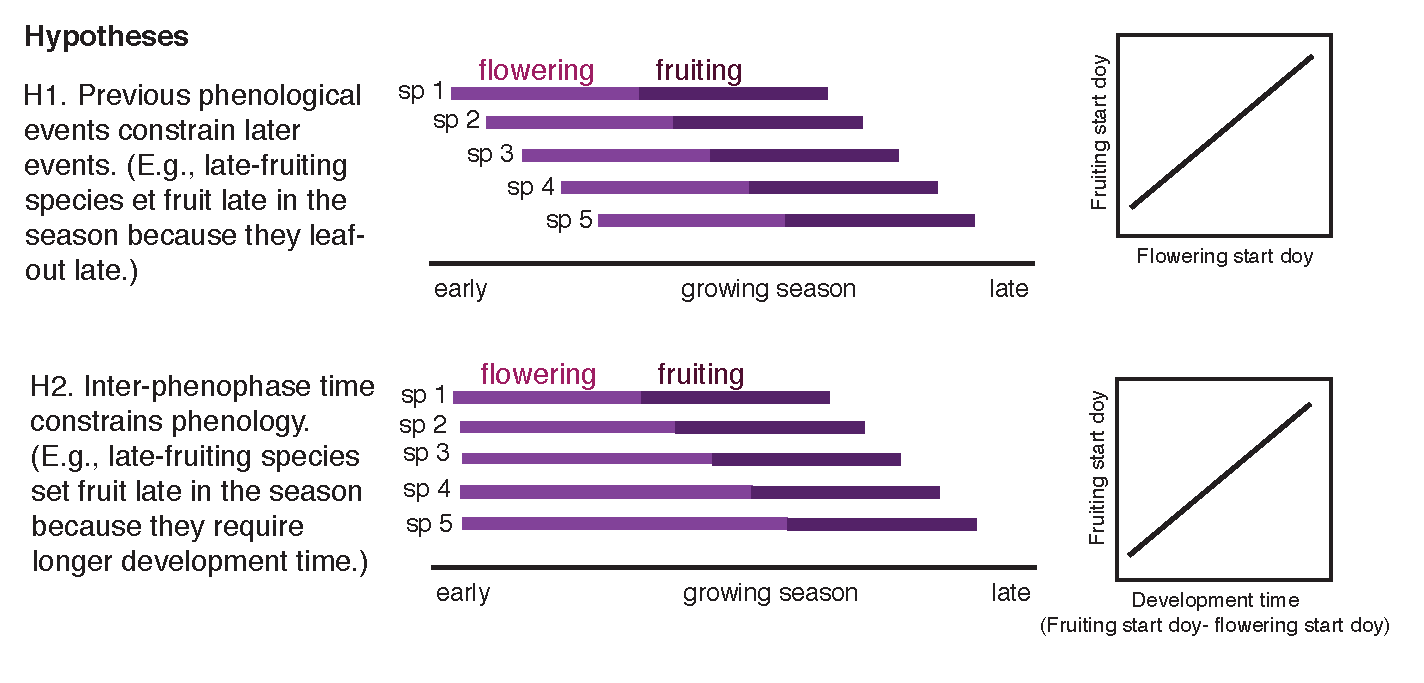
\includegraphics{../analyses/figures/hypotheses.pdf} 
  \caption{Hypotheses.} 
 \label{fig:hyp}
\end{figure}
 
\begin{figure}[h]
  \centering
  \includegraphics{../analyses/figures/grosea_errbars_1.jpeg}
  \caption{Focal species and their phenology.}
  \label{fig:focsp}
\end{figure}
  
  \begin{figure}[h]
  \centering
  \includegraphics{../analyses/figures/latevearly.pdf}
  \caption{Earlier phenological stages constrain later stages.}
  \label{fig:latevearly}
\end{figure}
\begin{figure}[h]
  \centering
  \includegraphics{../analyses/figures/adj_stagesmegaplot.pdf}
  \caption{Reproductive phenology is constrained by inter-phenophase time.}
  \label{fig:inter}
   \end{figure}
%%%%%%%%%%%%%%%%%%%%%%%%%%%%%%%%%%%%%%%%
\end{document}
%%%%%%%%%%%%%%%%%%%%%%%%%%%%%%%%%%%%%%%%
